% !TEX root = ../main.tex
\section{实验结果与分析}

\subsection{已知拓扑下的动力学学习性能}

首先考察网络已知时，模型能否从状态转移数据中恢复 SIR 的局部演化关系。
\cref{tab:known-main}给出五个模型在 ER、WS 和 BA 三类网络上的平均结果。
双向双通道模型的感染率反演误差、完整感染曲线误差、恢复率误差和自回归误差均为五者最低。
这组结果体现了双通道模型在预测、规律校准和多步推演之间的综合优势。

\begin{table}[H]
  \centering
  \caption{已知网络时五类学习器在 ER、WS、BA 上的平均结果}
  \label{tab:known-main}
  \begin{threeparttable}
  \begin{tabular}{@{}lccccc@{}}
    \toprule
    模型 & $|\hat\beta-0.3|$ & 逐 $k$ MAE & $|\hat\gamma-0.1|$ & $\Delta\gamma$ & 自回归 MAE(I) \\
    \midrule
    单向求和 GraphConv-1L & 0.09089 & 0.19924 & 0.00297 & 0.00719 & 0.03693 \\
    双向求和 GraphConv-1L & 0.07940 & 0.09188 & 0.00877 & 0.03437 & 0.03219 \\
    双向求和 GraphConv-3L & 0.02356 & 0.02730 & 0.00602 & 0.01039 & 0.01134 \\
    双向均值 GraphConv-3L & 0.02355 & 0.13654 & 0.00472 & \textbf{0.00050} & 0.01386 \\
    {\yahei 双向双通道} & \textbf{0.00406} & \textbf{0.01296} & \textbf{0.00234} & 0.00135 & \textbf{0.00789} \\
    \bottomrule
  \end{tabular}
  \end{threeparttable}
\end{table}

\cref{fig:known-results}进一步揭示了差异从何而来。
BA 网络包含少量高度数节点，最容易暴露聚合方式的问题。
均值聚合在中高邻居数区域给出的感染概率趋于平台，
说明感染邻居比例不能稳定替代绝对数量；
单向边表因遗漏部分消息而产生更明显偏差。
增加隐藏非线性后，
求和 GraphConv 已能恢复曲线的大致形状，
但双通道模型在不同节点度数上的响应更一致。
这说明分离表示能够减轻量级失衡和信息混合，
使局部交互响应更加稳定。

\begin{figure}[!htbp]
  \centering
  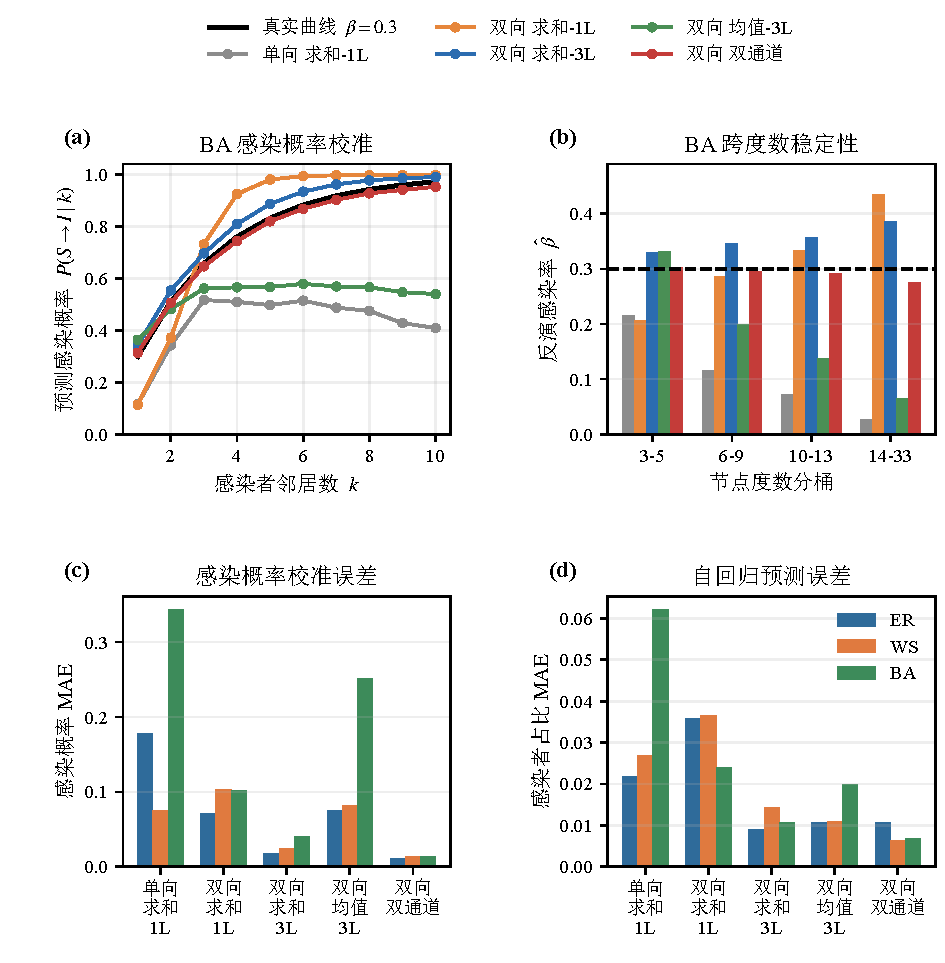
\includegraphics[width=\textwidth]{known_topology_results.pdf}
  \caption{已知网络时五类学习器的比较。
(a) BA 网络的感染概率曲线；
(b) BA 网络按节点度数得到的感染率反演；
(c) 三类网络的曲线误差；
(d) 三类网络的多步推演误差。}
  \label{fig:known-results}
\end{figure}

双通道模型在 ER、WS、BA 上反演得到的 $\hat\beta$ 分别为 0.3036、0.3079 和 0.3007，与真实值 0.3 接近；
逐 $k$ 误差分别为 0.0111、0.0137 和 0.0140。
其感染者占比自回归 MAE 分别为 0.0106、0.0063 和 0.0067，
表明一步规律在闭环推演中没有快速偏离。
三个网络上的感染响应与群体演化结果共同支持了分离表示对动力学学习的积极作用。

\subsection{未知拓扑下的网络重构性能}

进一步移除真实网络，只保留状态时间序列。
按照验证交叉熵选择的三个模型见\cref{tab:unknown-main}。
在该组固定实例上，
WS 网络被完整恢复；
BA 只多预测 4 条边；
ER 存在 41 条假阳性边和 24 条假阴性边，
但硬图 F1 仍达到 0.9374。
三类网络的 Precision 和 F1 均明显高于仅靠预测稠密网络可能得到的水平，
说明模型恢复的不只是能够参与计算的任意权重矩阵，
而是与真实连接高度一致的离散图。

\begin{table}[H]
  \centering
  \caption{未知网络时所选模型的拓扑恢复、参数诊断与多步推演结果}
  \label{tab:unknown-main}
  \resizebox{\textwidth}{!}{%
  \begin{tabular}{@{}lccccccccccc@{}}
    \toprule
    网络 & seed & 验证 CE & ACC & Precision & F1 & TPR & FPR & 边数 & $\hat\beta$ & $\hat\gamma\pm s$ & MAE(I) \\
    \midrule
    ER & 42 & 0.073868 & 0.9869 & 0.9223 & 0.9374 & 0.9530 & 0.0092 & 528/511 & 0.2942 & $0.1039\pm0.0028$ & 0.0072 \\
    WS & 7  & 0.074515 & 1.0000 & 1.0000 & 1.0000 & 1.0000 & 0.0000 & 300/300 & 0.2996 & $0.1008\pm0.0028$ & 0.0059 \\
    BA & 7  & 0.074649 & 0.9992 & 0.9864 & 0.9932 & 1.0000 & 0.0009 & 295/291 & 0.2889 & $0.1037\pm0.0022$ & 0.0082 \\
    \bottomrule
  \end{tabular}}
  \parbox{\textwidth}{\footnotesize\vspace{0.35em}注：$s$ 表示不同控制状态上模型输出的离散程度，
不是统计置信区间。}
\end{table}

\cref{fig:seed-recon}(a)展示全部九次优化及最低验证交叉熵选出的模型。
三个网络上，所选结果均位于较低验证损失与较高硬图 F1 的区域，
表明验证信号在本组实验中能够有效识别高质量候选网络。
图中同时保留其他初始化结果，
便于观察选模过程；
不同优化结果的差异及其机制在讨论部分分析。

\begin{figure}[!htbp]
  \centering
  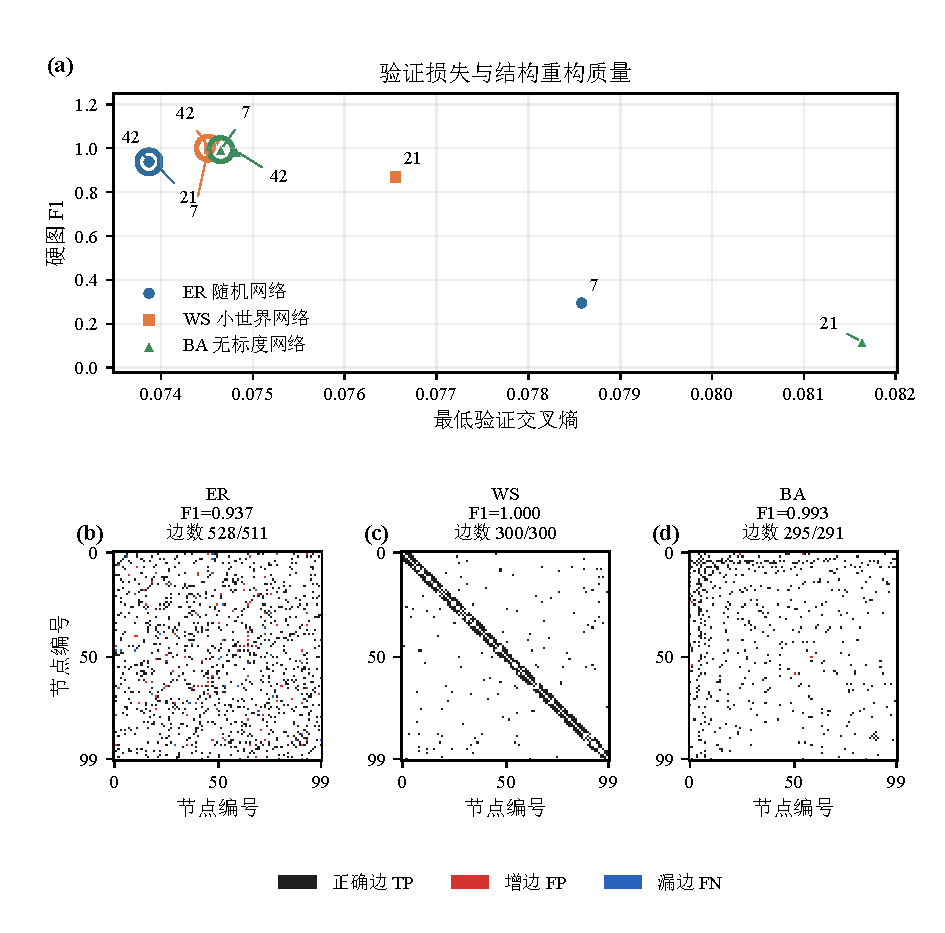
\includegraphics[width=\textwidth]{seed_selection_and_reconstruction.pdf}
  \caption{不同初始化与拓扑恢复结果。
(a) 九次训练的验证交叉熵和硬图 F1，数字为训练 seed，空心圆为所选模型；
(b)--(d) ER、WS、BA 所选硬图中的正确边、假阳性边和假阴性边。}
  \label{fig:seed-recon}
\end{figure}

软图 AUC 在三个所选模型上分别为 0.9863、1.0000 和 1.0000，但 AUC 只反映边分数的排序，不能说明固定阈值下会保留多少错误边。
本文因此把 Precision、F1 和预测边数作为结构结论的主要依据。
这一选择也体现了全文的基本判断：用于预测的连续关系分数与最终需要解释的离散网络并不是同一件事。

\subsection{参数反演与多步预测性能}

\cref{fig:calibration-autoreg}从参数诊断和多步推演两个层面展示重构网络对动力学预测的支持。
未知网络时，
ER、WS、BA 的感染率反演值分别为 0.2942、0.2996 和 0.2889，
恢复率反演值分别为 0.1039、0.1008 和 0.1037；
前者整体接近真实值 0.3，
后者接近真实值 0.1，
体现了所学局部响应与真实动力学的一致性。

\begin{figure}[!htbp]
  \centering
  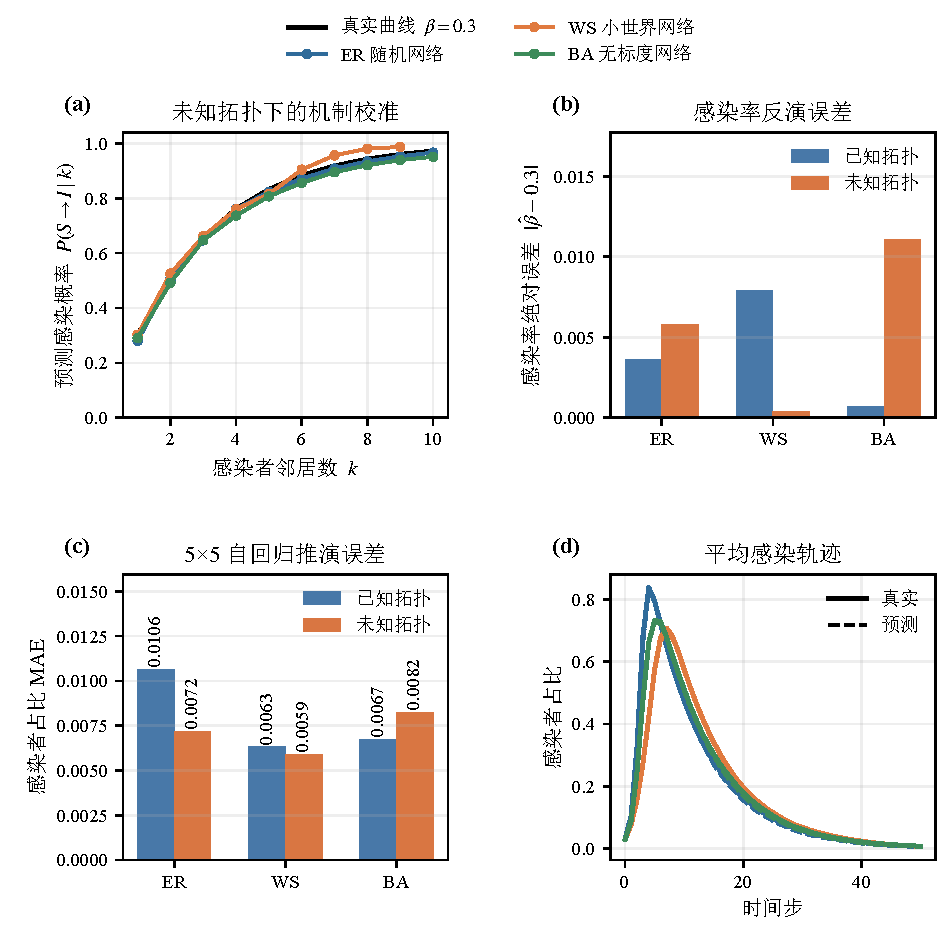
\includegraphics[width=\textwidth]{calibration_and_autoregression.pdf}
  \caption{规律诊断与多步推演。
(a) 未知网络时学习到的感染响应；
(b) 已知与未知网络下的感染率反演误差；
(c) 两阶段的感染者占比自回归误差；
(d) 未知网络模型在代表性初始条件下的平均感染者轨迹。
两阶段训练条件不同，
图中并列只用于比较误差量级。}
  \label{fig:calibration-autoreg}
\end{figure}

未知网络下三类模型的感染者占比自回归 MAE 为 0.00716、0.00588 和 0.00824，三状态平均 MAE 为 0.00609、0.00510 和 0.00886。
它们与已知网络双通道模型处在相近量级，
说明所恢复的连接能够支撑稳定的闭环演化，
而不仅是一次性的边集合匹配。
在本组实验条件下，
这些结果表明动力学规律与主要拓扑可以由同一组时间序列共同恢复。
\FloatBarrier
